%                                                                 aa.dem
% AA vers. 9.1, LaTeX class for Astronomy & Astrophysics
% demonstration file
%                                                       (c) EDP Sciences
%-----------------------------------------------------------------------
%
%\documentclass[referee]{aa} % for a referee version
%\documentclass[onecolumn]{aa} % for a paper on 1 column  
%\documentclass[longauth]{aa} % for the long lists of affiliations 
%\documentclass[letter]{aa} % for the letters 
%\documentclass[bibyear]{aa} % if the references are not structured 
%                              according to the author-year natbib style

%
\documentclass{aa}  
\usepackage{float}
%
\usepackage{multirow}
\usepackage{graphicx}
%%%%%%%%%%%%%%%%%%%%%%%%%%%%%%%%%%%%%%%%
\usepackage{txfonts}
%%%%%%%%%%%%%%%%%%%%%%%%%%%%%%%%%%%%%%%%
\usepackage[colorlinks=true,allcolors=blue]{hyperref}
% To add links in your PDF file, use the package "hyperref"
% with options according to your LaTeX or PDFLaTeX drivers.
%
\begin{document} 


   \title{Signatures of UV radiation around low-mass protostars in the Serpens Main with IRAM 30m}

   \subtitle{}

   \author{Agnieszka Mirocha\inst{1}$^,$\inst{2}
	  \and
          Agata Karska\inst{2}
	  \and
	  Lars E. Kristensen\inst{3}
	  \and
	  Marcin Gronowski\inst{4}
	  \and
	  Miguel Figueira\inst{5}
	  \and
	  Marcin Gładkowski\inst{2}$^,$\inst{6}
	  \and
	  Michał Żółtowski\inst{2}
          }

   \institute{Astronomical Observatory of the Jagiellonian University, ul. Orla 171, 30-244 Kraków, Poland\\
 	 \email{amirocha@doctoral.uj.edu.pl}
         \and Centre for Astronomy, Faculty of Physics, Astronomy and Informatics, Nicolaus Copernicus University, ul. Grudziądzka 5, 87-100 Toruń, Poland
         \and Centre for Star and Planet Formation, Niels Bohr Institute and Natural History Museum of Denmark, University of Copenhagen, Øster Voldgade 5-7, DK-1350 Copenhagen K, Denmark 
	 \and Faculty of Physics, University of Warsaw, ul. Pasteura 5, 02-093 Warszawa, Poland
	 \and National Centre for Nuclear Research, ul. Pasteura 7, 02-093 Warszawa, Poland
	 \and Nicolaus Copernicus Astronomical Center, ul. Rabiańska 8, 87-100 Toruń, Poland \\
         }

   \date{Received [Month] [Day], 2019; accepted [Month] [Day], 2019}

% \abstract{}{}{}{}{} 
% 5 {} token are mandatory
 
  \abstract
  % context heading (optional)
  % {} leave it empty if necessary  
   {The Serpens Main is one of the most studied star forming region containing low-mass protostars. Observations at submillimetre range allow to determine physical and chemical processes around young stellar objects.} %especially HCN and CN have been shown to be good tracers of photon dominated regions (PDR}.
  % aims heading (mandatory)
   {We aim to characterise the UV radiation in the surroundings of the low-mass protostars. We analyse the exitation and spatial extend of HCN, CN, CS and their isotopologues to identify the underlying processes. We can investigate the feedback from protostars and the excitation mechanism of molecules. }
  % methods heading (mandatory)
   {We present ~30 arcmin$^2$ IRAM 30m maps of CN $J=1-0$, HCN $J=1-0$, and CS $J=3-2$ encompassing 10 low-mass protostars. We calculated HCN $J=1-0$ and CN $J=1-0$ column densities around low-mass protostars and selected outflows positions using the RADEX radiative transfer code.  The obtained column densities were compared with the astrochemical model of molecules abundaces in order to characterise UV radiation field.}
  % results heading (mandatory)
   {Emission of HCN $J=1-0$ and CS $J=3-2$ is co-spatial with outflows, CN emission peaks at the positions of protostars. CN $J=1-0$ and HCN $J=1-0$ column densities were estimated as 10$^{13}$-10$^{14}$cm$^{-2}$. Regardless of gas parameters CN/HCN column density ratio was modeled in range of 1-10. This result can be reproduced by providing an additional UV radiation source of 0.044 to 0.001 $G_0$.}
  % conclusions heading (optional), leave it empty if necessary 
   {As a product of HCN photodissociation CN molecules indicate bow shocks around young stellar objects. The astrochemical model obtained with the Nahoon code shows that an additional source of UV radiation is needed to cover the abundances range indicated by observations.}

   \keywords{astrochemistry -- stars: formation -- ISM: molecules -- ISM: individual objects: Sepens Main -- Submillimeter: ISM}

   \maketitle
%
%-------------------------------------------------------------------

\section{Introduction}


\section{Observations}
The Serpens Main star forming region was observed with IRAM 30 between 14 and 17 July 2009 (project no. xxx, PI: L. Kristensen). We used the Eight MIxer Receiver (EMIR) as the frontend. The observations were performed in the EMIR bands E090 (molecule HCN $J=1-0$) covering the range 73-117 GHz and E150 (molecules CN $J=1-0$ and CS $J=3-2$) covering the frequencies between 125 and 184 GHz. Due to the EMIR receiver wide bands additional molecular lines of C$^{34}$S $J=3-2$, H$^{13}$CN $J=1-0$ and H$^{13}$CN $J=2-1$ were also observed. The backend was the Versatile SPectrometer Array (VESPA) autocorrelator and the 1 MHz filterbank reaching the spectral resolution of 39 kHz (E150 band) and 78 kHz (E090 band). The telescope beam size varies from 14$^{\prime\prime}$ at 172.68 GHz to 29$^{\prime\prime}$ at 86.34 GHz (Table 1). The antenna temperatures were converted to main-beam brightness temperature \textit{T$_\mathrm{MB}$} using the main beam efficiency according to the expresion: T$_\mathrm{MB}$ = T$_\mathrm{A}$/$\eta_\mathrm{MB}$. The exact upper levels enegies, line frequencies, beam sizes and beam efficiencies are given in Table~\ref{table:1}. Observations included scans of the Ser-SMM1 (centered at $\alpha_\mathrm{J2000}$ = 18$^h$29$^m$49.6$^s$, $\delta_\mathrm{J2000}$ = +01$^{\circ}$15$^{\prime}$20.5$^{\prime\prime}$ with V$_\mathrm{LSR}$ = +8.5 km/s) and the Ser-SMM3/Ser-SMM4 (centered at $\alpha_\mathrm{J2000}$ = 18$^h$29$^m$56.6$^s$, $\delta_\mathrm{J2000}$ = +01$^{\circ}$14$^{\prime}$00.3$^{\prime\prime}$ with V$_\mathrm{LSR}$ = +7.6 km/s) regions, both 1$^{\prime}\times$3$^{\prime}$ OTF maps. The size of the maps is about 300$^{\prime\prime}\times350^{\prime\prime}$, covering both Ser-SMM1 and Ser-SMM3/Ser-SMM4 regions. The regions are referenced in the article as 'the Northen part' and 'the Southern part' respectively. 

\begin{table}
\caption{Overview of the observations}             % title of Table
\label{table:1}      % is used to refer this table in the text
\centering                          % used for centering table
\begin{tabular}{c c c c c c}        % centered columns (4 columns)
\hline\hline                 % inserts double horizontal lines
Mol. & Trans. & $E_\mathrm{u}$ & Freq. &  Beam size & Beam eff.\\
 & & (K) & (GHz) & ($^{\prime\prime}$) & $\eta_\mathrm{MB}$\\
\hline                        % inserts single horizontal line
HCN & 1-0 & 4.25 & 88.631602 & 28 & 0.81\\
CN & 1-0 & 5.45 & 113.494921 & 22 & 0.78\\
CS & 3-2 & 14.1 & 146.969029 & 16 & 0.74\\
C$^{34}$S & 3-2 & 13.9 & 144.617109 & 16 & 0.74\\
H$^{13}$CN & 1-0 & 4.14 & 86.342274 & 29 & 0.81\\
H$^{13}$CN & 2-1 & 12.43 & 172.677881 & 14 & 0.68\\
\hline                                   
\end{tabular}
\tablefoot{Beam sizes and efficiencies are taken from \url{http://www.iram.es/IRAMES/mainWiki/Iram30mEfficiencies}}
\end{table}

Data reduction was carried out with the CLASS package within GILDAS\footnote{See http://www.iram.fr/IRAMFR/GILDAS}. Each spectrum was corrected for the baseline shape, the spike channels were removed and the velocity was resampled to a resolution of 0.5 km/s. The baseline fitting of the order of 0 was sufficient for our observations. The rms of extracted spectra values vary from 0.024 K to 0.125 K. Both OTF maps were merged in one map covering 300$\times$350 arcsec. The spectra obtained were exported from the CLASS package and analysed with Python scripts. 


\section{Results}

\subsection{Physical properties of embedded protostars}
Ten Class 0/I protostars are present in the observed region. Spectral Energy Disribution (SED) was obtain for each of observed protostars in order to determine its properties. 

Most of the protostars in our sample have not been investigated for their properties after \textit{Herschel} observations. Only SMM1, SMM3 and SMM4 were covered by PACS spectroscopy as part of the WISH and DIGIT team surveys (Karska et al. 2013). Based on literature samples the data from the Herschel Gould Belt survey (HGBS) project (André et al. 2010) we re-calculated SEDs for those sources (Fig.~\ref{seds}).

The linear interpolation was performed while calculating the protostars parameters. The bolometric luminosity was determined by integrating the SEDs over frequency:
\begin{equation} \label{eq1}
L_{bol} = \pi \, d^2 \, \int F_\nu d\nu
\end{equation}
where $d$ is the cloud distance of 436 \pm 9.2 pc (Ortiz-León et al. 2017).
The bolometric temperature was calculating as described in Myers and Ladd 1993:
\begin{equation} \label{eq2}
T_{bol} = 1.25 \, 10^{-11} \, \bar{\nu}
\end{equation}
where $\bar{\nu}$ is the mean frequency given by:
\begin{equation} \label{eq3}
\bar{\nu} = \frac{\int \nu F_\nu d\nu}{ \int F_\nu d\nu}
\end{equation}

Table~\ref{table:2} contains the observed protostars parameters as well as the Class classification. The classification was adopted from Enoch et al. 2009 where four types of protostars with envelopes were distinguished. Early Class 0 was defined as a protostar of bolometric temperature lesser than 50 K. Prostostars characterised by bolometric temperature between 50 K and 100 K were classified as Late Class 0 protostars. Class I protostars were divided for Early and Late sub-type by the bolometric temperature of 300 K.

Most of the observed protostars in the Serpens Main region are very young, embedded sources of Early Class 0. SMM5 and SMM12 were classified as Early Class I YSOs. The SMM6 protostar is the most evolved object in our sample. 

\begin{figure}
   \includegraphics[width=8cm]{serpens_seds.eps}
      \caption{Serpens Main protostars' spectral energy distribution. There is an offset between plots of 3.0 $W m^{-2} s^{-1}$.}
         \label{seds}
   \end{figure}


\begin{table*}
\caption{Catalogue of protostars properties}             % title of Table
\label{table:2}      % is used to refer this table in the text
\centering                          % used for centering table
\begin{tabular}{c c c c c c c} 
\hline\hline 
R.A. & Decl. & Sbmm source & Other names & $T_\mathrm{bol}$ &  $L_\mathrm{bol}$  & Class\\
 (J2000.0) & (J2000.0) & & & (K) & (L$_\odot$) & \\
\hline  

18 29 48.3 & +01 16 42.7 & SMM9 & ISO241, WMW23& 46.14 & 11.69 & Early Class 0\\

18 29 50.0 & +01 15 20.3 & SMM1 & FIRS1, Ser-emb6, Bolo23, EC41 & 40.35 & 108.72 & Early Class 0\\

18 29 51.4 & +01 16 38.3 & SMM5 & EC53, WMW24, Ser p3 & 148.24 & 4.49 & Early Class I\\

18 29 52.3 & +01 15 48.8 & SMM10 & WMW21 & 85.09 & 5.13 & Late Class 0\\

18 29 57.0 & +01 13 11.3 & SMM4 & & 29.54 & 13.6 & Early Class 0\\

18 29 57.8 & +01 14 05.3 & SMM6 & EC90, WMW35, SVS20S & 526.44 & 43.39 & Late Class I\\

18 29 59.1 & +01 13 14.3 & SMM12 & & 100.87 & 6.68 & Early Class I\\

18 29 59.6 & +01 13 59.2 & SMM3 & & 42.39 & 27.49 & Early Class 0\\

18 30 00.5 & +01 12 57.8 & SMM2 & Ser-emb4, Bolo28 & 41.6 & 5.1 & Early Class 0\\

18 30 01.9 & +01 15 09.2 & SMM8 & & & 0.068$^a$ & \\
\hline
\end{tabular}
\begin{flushleft}
Coordinates taken from Suresh et al. 2016, except S68N (Enoch et al. 2007) and SMM8 (Lee et al. 2014).\\
References: $a$ Dionatos et al. 2010
\end{flushleft}
\end{table*}

\subsection{Molecular emission maps}

The line maps in the targeted molecules show variety of structures that can be associated with YSOs and a large-scale cloud emission. In the following section we present the large-scale maps of CS $J=3-2$, HCN $J=1-0$ and CN $J=1-0$. Similar maps are shown in the Appendix A.

The integrated line intensity map of HCN $J=1-0$ is shown in Fig.~\ref{hcn10}. 
Thirteen low-mass protostars can be distinguished in the field of view. Their positions and properties are shown in Table~\ref{table:2} \footnote{The outflows associated with low-mass protostars were obtained based on CO $J=6-5$ and CO $J=3-2$ observations (Y{\i}ld{\i}z et al. 2015)}. We have chosen six off-source positions where HCN $J=1-0$ or CN $J=1-0$ have the maximum of emission at the location of outflows. Their coordinates and short descriptions is presented in Table~\ref{table:3}.



\begin{table}
\caption{Properties of the selected off-source positions}             % title of Table
\label{table:3}      % is used to refer this table in the text
\centering                          % used for centering table
\begin{tabular}{c c c c} 
\hline\hline 
Pos. & R.A. & Decl. & Remarks\\
 & (J200) & (J200) & \\
\hline
1 & 18:29:45.47 & +01:15:53.5 & SMM1 blue-shifted \\
 & & & outflow in CO $J=3-2$\\
\hline
2 & 18:29:54.66 & +01:13:19.5 & max. CN $J=1-0$, \\
 & & & SMM4 blue-shifted \\
 & & & outflow in CO $J=3-2$\\
\hline
3 & 18:29:50.33 & +01:13:68.5 & max. HCN $J=1-0$, \\
 & & & SMM4 blue-shifted \\
\hline
4 & 18:29:43 & +01:16:41.5 & outflow visible \\
 & & &  in C$^{34}$S(3-2)\\
\hline
5 & 18:29:56.13 & +01:14:14.5 & max. CN $J=1-0$, \\
 & & & SMM9 surroundings\\
\hline
\end{tabular}
%\begin{flushleft}
%$a$ Y{\i}ld{\i}z et al. 2015 \\
%\end{flushleft}
\end{table}

There is no intensively elongated outflow structure from Ser-SMM3 source. The HCN $J=1-0$ map shows extended emission along outflow directions. The HCN $J=1-0$ line was detected at all positions, although it is weak at the positions of Ser-SMM5 and Ser-SMM10. On the other hand, the HCN $J=1-0$ emission is particularly strong around Ser-SMM4 and Ser-SMM9 sources. The emission maxima are detected among the known outflows of Ser-SMM1 and Ser-SMM4 (Y{\i}ld{\i}z et al. 2015). Especially, at the end of Ser-SMM4 blue outflow (position no. 4) we have significantly strong maximum of the HCN $J=1-0$ radiation. 

\begin{figure}
   \centering
   \includegraphics[width=8cm]{serpens_hcn10.eps}
      \caption{Emission of the HCN $J=1-0$ in the Serpens Main region. Black triangles show the positions of the protostars (Suresh et al. 2016), whereas the black lines show the associated outflow directions (Y{\i}ld{\i}z et al. 2015). Outflow positions were displayed as pulrple crosses.}
         \label{hcn10}
   \end{figure}

CS $J=3-2$ line emission map shows similar spatial distribution to HCN $J=1-0$ (Fig.~\ref{cs32}). The most significant elongated structure can be associated with Ser-SMM4 blue-shifted outflow. It is situated at the same place in both maps, extending over 80$^{\prime\prime}$. A similar large-scale structure is detected along Ser-SMM1 outflows, although it is much more distinctive in the HCN $J=1-0$ map. A strong emission around Ser-SMM9 have a circular shape in HCN $J=1-0$ map, however, it has more elongated structure in CS $J=3-2$ line emission which overlaps with the S68N outflows (Kristensen et al. 2010). The peaks of emissions are situated in the different places. HCN $J=1-0$ has relatively strong emission around Ser-SMM4 protostar, but in CS $J=3-2$ line a significant emission towards position no. 3 can be noticed that indicates CN $J=1-0$ local maximum. 

CN $J=1-0$ line emission is focused mostly around the positions of protostars (Fig.~\ref{cn10}). 
The highest local peaks are associated with Class 0 low-mass protostars: Ser-SMM1 (8.2~K~km/s), Ser-SMM3 (15.9~K~km/s), Ser-SMM4 (14.1~K~km/s) and Ser-SMM6 (15.3~K~km/s). The spatial distribution is qualitatively different compared to the HCN $J=1-0$ map. The strongest emission characterises the dense surroundings of Ser-SMM3, Ser-SMM6 and Ser-SMM4 sources while the northern part of this region does not show such a distinct emission in the HCN $J=1-0$ line. On the other hand, dense emissive region of the Ser-SMM9 source is significantly weaker in CN $J=1-0$ line. CN $J=1-0$ map can be characterised by compact, condensed emission without any strongly elongated structures. The H$^{13}$CN $J=1-0$ line exhibits similar morphological distribution as CN(1-0) and \mbox{C$^{34}$S(3-2)}. 

In the presence of the UV radiation, HCN molecule photodissociates into CN molecule and H atom (Stäuber et al. 2005). Thus, combined map of these molecules can indicate regions with stronger UV radiation. We present a large-scale map of CN $J=1-0$ to HCN $J=1-0$ flux ratio (Fig.~\ref{cn10_div_hcn10}). The image of CN emission has been resampled to beam size of HCN in order to compare the same emitting regions. CN/HCN ratio is relatively low around the brightest submillimetre source Ser-SMM1. Similarly, at the dense area of Ser-SMM9 surrounding a significantly weaker CN/HCN emission can be noticed. On the other hand, it peaks at the Northern part of the map around rather faint Ser-SMM5 source. At the Southern part high CN/HCN ratio emission is more extended than in the Northen part. It expands from Ser-SMM3 and Ser-SMM6 area to the North. High CN/HCN ratio can also be found on the edges of the image but it is probably caused by different size of the CN and the HCN maps.

\begin{figure}
   \centering
   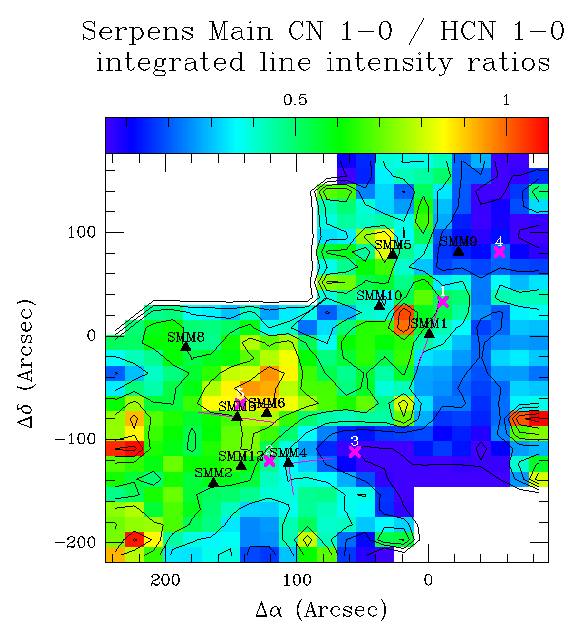
\includegraphics[width=8cm]{serpens_cn10_divided_hcn10.eps}
      \caption{Emission of the divided fluxes CN $J=1-0$/HCN $J=1-0$ in the Serpens Main region. Black triangles show the positions of the protostars (Suresh et al. 2016), whereas the black lines show the associated outflow directions (Y{\i}ld{\i}z et al. 2015). Outflow positions were displayed as pulrple crosses.}
         \label{cn10_div_hcn10}
   \end{figure}

The low energy level of HCN ($E_\mathrm{u}$ = 4.25 K) traces cold, high-density gas. HCN has previously been shown to be a good tracer of molecular outflows activity (Walker-Smith et al. 2014). Similar spatial distribution is presented in the CS map. It means that both species trace the gas of the same properties. The CN line is similarly low-energetic, however it peaks in different areas than HCN and CS. CN as a product of HCN photodissotiation indicates other properties of low-mass protostars surroundings (Section 4).

To summarise, spatial distribution of different lines emission varies depending on the observed molecule. The most distinct differences can be noticed between HCN and CN map. Most of the sources show high flux values in both molecules (Table~\ref{table:4}). However, they present unequal levels which indicates regions of different properties. In order to better understand this issue we analyse the molecular line profiles in the Section 3.2. 

\begin{table}
\caption{Integrated fluxes of the detected protostars}             % title of Table
\label{table:4}      % is used to refer this table in the text
\centering                          % used for centering table
\begin{tabular}{c c c c c} 
\hline\hline 
Source & Line & Line freq.$^a$ & Flux$^b$ & Column dens. \\
 &  & (MHz) & (K) & (cm$^{-2}$) \\
\hline  
\multirow{6}{*}{SMM1} & CN 1-0 & 113487.66 & 6.53 & 1.3$\times$10$^{15}$\\
{} & HCN 1-0 & 88629.53 & 6.78 & 1.9$\times$10$^{14}$ \\ 
{} & CS 3-2 & 146964.15 & 6.93 & 7.9$\times$10$^{13}$\\  
{} & C$^{34}$S 3-2 & 144612.88 & 1.39 & 1.7$\times$10$^{13}$\\ 
{} & H$^{13}$CN 1-0 & 86337.74 & 1.28 & no data\\ 
{} & H$^{13}$CN 2-1 & 172708.89 & 0.03 & no data\\  \hline
\multirow{6}{*}{SMM2} & CN 1-0 & 113488.17 & 10.58 & 2.2$\times$10$^{15}$ \\
{} & HCN 1-0 & 88629.77 & 13.98 & 4.0$\times$10$^{14}$\\ 
{} & CS 3-2 & 146965.22 & 8.03 & 9.1$\times$10$^{13}$\\  
{} & C$^{34}$S 3-2 & 144613.51 & 1.15 & 1.4$\times$10$^{13}$\\
{} & H$^{13}$CN 1-0 & 86337.94 & 2.46 & no data\\ 
{} & H$^{13}$CN 2-1 & \multicolumn{3}{c}{not detected}  \\  \hline
\multirow{6}{*}{SMM3} & CN 1-0 & 113488.19 & 13.26 & 2.7$\times$10$^{15}$\\
{} & HCN 1-0 & 88629.61 & 12.48 & 3.6$\times$10$^{14}$\\ 
{} & CS 3-2 & 146966.10 & 10.04 & 1.1$\times$10$^{14}$\\  
{} & C$^{34}$S 3-2 & 144613.41 & 0.37 & 4.4$\times$10$^{12}$\\
{} & H$^{13}$CN 1-0 & 86337.92 & 0.98 & no data\\ 
{} & H$^{13}$CN 2-1 & \multicolumn{3}{c}{not detected}  \\  \hline
\multirow{6}{*}{SMM4} & CN 1-0 & 113488.05 & 13.06 & 2.7$\times$10$^{15}$\\
{} & HCN 1-0 & 88629.61 & 20.20 & 5.7$\times$10$^{14}$ \\ 
{} & CS 3-2 & 146965.44 & 19.81 & 2.2$\times$10$^{14}$\\  
{} & C$^{34}$S 3-2 & 144613.74 & 0.02 & 1.9$\times$10$^{11}$\\ 
{} & H$^{13}$CN 1-0 & 86337.80 & 2.10 & no data\\ 
{} & H$^{13}$CN 2-1 & 172673.09 & 0.26 & no data\\  \hline
\multirow{6}{*}{SMM5} & CN 1-0 & 1113488.05 & 2.57 & no data\\
{} & HCN 1-0 & 88629.53 & 3.71 & 1.1$\times$10$^{14}$\\ 
{} & CS 3-2 & 146965.03 & 2.33 & no data\\  
{} & C$^{34}$S 3-2 & 144613.14 & 0.07 & 7.9$\times$10$^{11}$\\ 
{} & H$^{13}$CN 1-0 & 86337.76 & 0.70 & no data\\ 
{} & H$^{13}$CN 2-1 & \multicolumn{3}{c}{not detected}  \\  \hline
\multirow{6}{*}{SMM6} & CN 1-0 & 113487.76 & 11.48 & 2.4$\times$10$^{15}$\\
{} & HCN 1-0 & 88629.61 & 11.85 & 3.4$\times$10$^{14}$ \\ 
{} & CS 3-2 & 146965.03 & 9.37 & 1.1$\times$10$^{14}$ \\  
{} & C$^{34}$S 3-2 & 144613.25 & 0.54 & 6.4$\times$10$^{12}$ \\ 
{} & H$^{13}$CN 1-0 & 86336.53 & 0.16 & no data\\
{} & H$^{13}$CN 2-1 & 172673.69 & 0.02 & no data \\  \hline
\multirow{6}{*}{SMM9} & CN 1-0 & 113487.64 & 4.82 & 9.9$\times$10$^{14}$\\
{} & HCN 1-0 & 88628.98 & 12.55 & no data \\ 
{} & CS 3-2 & 146963.87 & 13.75 & no data\\ 
{} & C$^{34}$S 3-2 & 144612.96 & 1.17 & 1.4$\times$10$^{13}$ \\ 
{} & H$^{13}$CN 1-0 & 86337.65 & 1.61 & no data\\ 
{} & H$^{13}$CN 2-1 & 172673.14 & 0.04 & no data\\  \hline
\multirow{6}{*}{SMM10} & CN 1-0 & 113487.58 & 2.89 & 5.9$\times$10$^{14}$\\
{} & HCN 1-0 & 88629.53 & 4.40 & 1.3$\times$10$^{14}$\\ 
{} & CS 3-2 & 146965.06 & 4.47 & 5.1$\times$10$^{13}$ \\  
{} & C$^{34}$S 3-2 & 1144613.19 & 0.35 & 4.2$\times$10$^{12}$\\ 
{} & H$^{13}$CN 1-0 & 86337.72 & 0.98 & no data\\ 
{} & H$^{13}$CN 2-1 & \multicolumn{3}{c}{not detected}  \\  \hline
\multirow{6}{*}{SMM12} & CN 1-0 & 113488.17 & 10.58 & 2.2$\times$10$^{15}$\\
{} & HCN 1-0 & 88629.77 & 13.98 & 4.0$\times$10$^{14}$\\ 
{} & CS 3-2 & 146965.06 & 10.30 & 1.2$\times$10$^{14}$\\  
{} & C$^{34}$S 3-2 & 144613.39 & 0.93 & 1.1$\times$10$^{13}$\\ 
{} & H$^{13}$CN 1-0 & 86337.94 & 2.46 & no data\\ 
{} & H$^{13}$CN 2-1 & \multicolumn{3}{c}{not detected}  \\  \hline
\end{tabular}
\begin{flushleft}
$a$ Line frequency at the main peak position. \\
$b$ Integrated flux above 3$\sigma$.\\
\end{flushleft}
\end{table}

\subsection{Line profiles}

\begin{figure*}
   \centering
   \includegraphics[width=15cm]{serpens_spectra_1.eps}
      %\caption{Serpens Main sources spectra of CS(3-2), HCN(1-0) abd CN(1-0) lines.}
         \label{Spectra_1}
   \end{figure*}
\begin{figure*}
   \centering
   \includegraphics[width=15cm]{serpens_spectra_2.eps}
      \caption{Serpens Main sources spectra of C$^{34}$S $J=3-2$, CS $J=3-2$, H$^{13}$CN $J=1-0$, HCN $J=1-0$ and CN $J=1-0$ lines.}
         \label{Spectra_1}
   \end{figure*}

We selected 14 representative on-source and off-source positions for a detailed analysis (Fig.~\ref{Spectra_1}). Nine of them are corresponding to the protostars positions, the other five off-source positions were selected based on local maximum of the flux.   

The mean region is consistent with HCN $J=1-0$ beam size (27.8") for all molecules. In the majority of our sources five of targeted lines were detected: CN $J=1-0$, HCN $J=1-0$, CS $J=3-2$, C$^{34}$S $J=3-2$ and H$^{13}$CN $J=1-0$. The line is considered to be detected if there is an emission at the level of at least 3$\sigma$. A weak emission from H$^{13}$CN $J=2-1$ was found at the positions of four sources and it is not included in the Figure. 

The strongest emission occurs in HCN $J=1-0$, CN $J=1-0$ and CS $J=3-2$ lines and it was detected at the position of all of the sources. The emission in the other lines was multiplied in order to compare profiles between different molecules. In HCN, CN species and their isotopologues a few different velocity components can be identified what indicates the hyperfine splitting. This occurs if a molecule has a non-zero nuclear spin so there is also an interaction between the nuclear spin and the electronic angular momentum. The most distinct splitting can be spotted in the CN $J=1-0$ profiles with five separate components situated between -70 km/s and 18 km/s. The HCN $J=1-0$ line is characterised by three components with low separation situated in the range of -2 km/s – 16 km/s. 

Ser-SMM1, Ser-SMM9, and Ser-SMM10 sources have wide spectral lines, while others exhibit narrow line profiles. Spectra extracted form Positions no. 1, 4 and 5 shows prominent blue-shifted wings what can be associated with outflows. Similar structure can be noticed in the Ser-SMM3 (panel no. 7) CS 3-2 and HCN $J=1-0$ profiles. 

\section{Analysis}

\subsection{Lines column densities}

Table 4 shows fluxes integrated from the average line profile at the positions of known protostars. 
Flux calculation in individual lines allows us to determine the column density of a given transition. The column density of the upper level $N_\mathrm{up}$ of each observed line was calculated based on following relation:
\begin{equation} \label{eq1}
N_u = \beta \, \frac{\nu \, W}{A}
\end{equation}
where $\beta$ = 1937 cm$^{-2}$ and $W = \int{T_{mb} \, dV}$ is the integrated intensity of the emission line. The frequency $\nu$ should be given in GHz.

The column densities of the upper level of CN $J=1-0$ and HCN $J=1-0$ transitions are presented in Table 4. In the closest surroundings of low-mass protostars CN $J=1-0$ is stronger than the lowest transition line of HCN. The column density of CN $J=1-0$ varies between 10$^{14}$ -10$^{15}$ cm$^{-2}$, while in the column density of the HCN’s lowest transition reaches 10$^{14}$ cm$^{-2}$ . Except for the Ser-SMM9 and the Ser-SMM10 neighbourhood, HCN $J=1-0$ line column density is an order of magnitude lower than the column density of the equivalent CN transition. This result provides a clue to better understand of the low-mass protostars chemistry.  

\subsection{RADEX modelling}

\begin{figure}
   \centering
   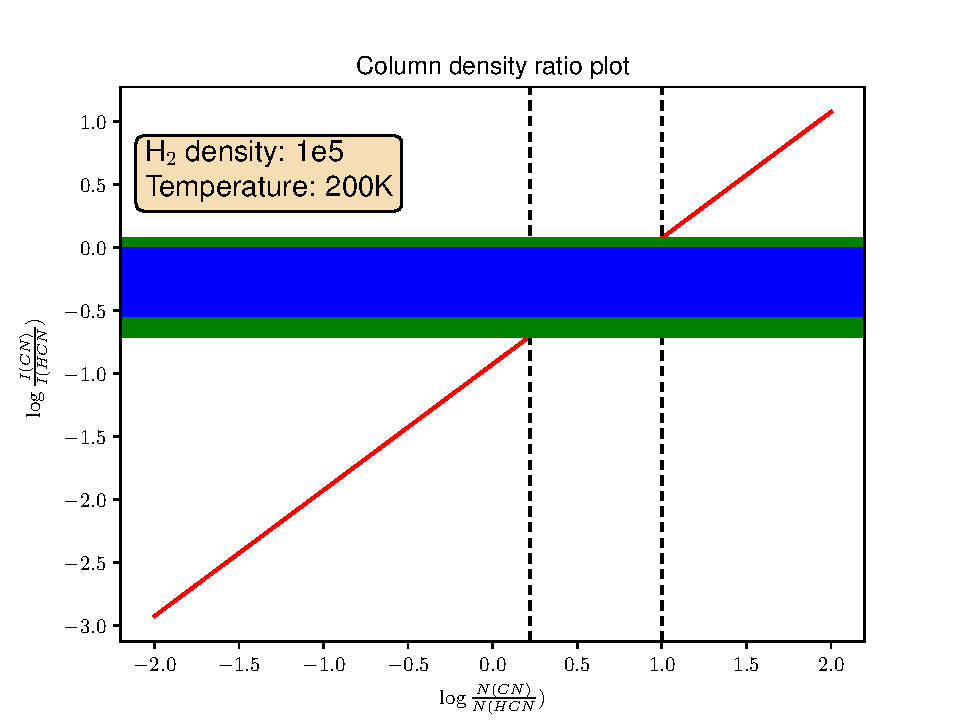
\includegraphics[width=10cm]{Nratios_plot_nH2-1e5_200K.eps}
      \caption{RADEX model predictions for the CN/HCN column density ratio for hydrogen densities of $n_\mathrm{H_2} = 10^5$ cm$^{-3}$ and kinetic temperatures of $T_\mathrm{kin} = 200$ K (red line). The observed line intensity ratio is plotted in blue (protostars positions) and green (all positions).}
         \label{1e5_75K}
   \end{figure}

Molecules column densities can be independently determined using molecular excitation models. Line ratio can provide additional information concerning physical properties of the observed gas. 

The non-LTE radiative transfer code RADEX (van der Tak et al. 2007) was run in order to prepare sets of molecular excitation models. The CN and HCN molecules column density ratio was the only free parameter. HCN column density was chosen as 10$^8$ cm$^{-2}$ in order to ensure optically thin emission. CN column density parameter varies from 10$^6$ cm$^{-2}$ to 10$^{10}$ cm$^{-2}$ what translates into $N_\mathrm{CN}$/$N_\mathrm{HCN}$ in following limits: 10$^{-2}$-10$^{2}$. The sets of models were developed assuming a line width of 1.0 km s$^{-1}$, hydrogen densities of $n_\mathrm{H_2} = 10^3$ cm$^{-3}$, $n_\mathrm{H_2} = 10^4$ cm$^{-3}$ and $n_\mathrm{H_2} = 10^5$ cm$^{-3}$ and kinetic temperatures of $T_\mathrm{kin} = 30$ K, $T_\mathrm{kin} = 75$ K and $T_\mathrm{kin} =200$ K. The molecular data files used during modelling were procured from the Leiden Atomic and Molecular Database (LAMDA, Schöier et al. 2005).

Fig.~\ref{1e5_75K} presents one exemplary set of models of CN/HCN column density ratio versus the modelled line intensities ratio for hydrogen densities of $n_\mathrm{H_2} = 10^5$ cm$^{-3}$ and kinetic temperatures of $T_\mathrm{kin} = 200$ K. The rest of the models are shown in the Appendix B. CN/HCN column density ratio weakly depends on hydrogen density and kinetic temperature in the low limit of those parameters. All presented models show similar properties.

The modelled line intensities are compared with the observations. The observed line intensity ratio covers a range of \mbox{0.0-1.0} of the column density ratio in the logarithmic scale. That corresponds to a few times higher CN column density than the same parameter of HCN. This result slightly depends on hydrogen densities and kinetic temperature of the gas (see Table~\ref{table:5}).

\begin{table}
\caption{CN and HCN column density ratio}             % title of Table
\label{table:5}      % is used to refer this table in the text
\centering                          % used for centering table
\begin{tabular}{c c c} 
\hline\hline  
$n_\mathrm{H_2}$ & $T_\mathrm{kin}$ & log$_{10}$(N[CN]/N[HCN]) \\
$[$cm$^{-3}]$ & [K] & \\
\hline
10$^{3}$ & 30 & 0.03-0.88\\
10$^{3}$ & 75 & 0.06-0.84\\
10$^{3}$ & 200 & 0.00-0.78\\ 
10$^{4}$ & 30 & 0.16-0.94\\
10$^{4}$ & 75 & 0.08-0.86\\
10$^{4}$ & 200 & 0.04-0.82\\ 
10$^{5}$ & 30 & 0.20-0.98\\
10$^{5}$ & 75 & 0.18-0.86\\
10$^{5}$ & 200 & 0.22-1.00\\ \hline
\end{tabular}
\end{table} 

The sets of models shown in this section indicate that CN/HCN column density ratio covers the range of 1-10 regardless of excitation conditions. This result suggests that the UV radiation may play an important role around low-mass protostars. 

\subsection{Astrochemical model}
In Section 4.2 we have raised a question about influence of the UV radiation on the surrounding of the observed sources. A simply astrochemical model can be obtained in order to estimate the intensity of the UV field in reference to units of the interstellar UV field $G_0$.

HCN easily photodissotiates into CN molecule and H atom. On the other hand, CN needs more energetic photon for disintegration. In the presence of the UV photons HCN can be dissociated, while CN cannot. This leads to higher abundance of CN molecules and increases CN/HCN column density ratio.

We used Nahoon code (Wakelam et al. 2012) that model the time evolution of 474 species involving gas-phase and gas-grain reactions with fixed temperature, density, UV, and cosmic ray fluxes. The evolution of CN, HCN and CS abundances was started at the time of a dense cloud formation. The UV radiation is described in the code by $A_\mathrm{V}$ parameter through the relation between visual extinction and the photodissociation rate coefficient:
\begin{equation} \label{eq1}
k =  \alpha e^{-\gamma A_\mathrm{V}}
\end{equation}
where $\mathrm{\alpha}$ and $\mathrm{\gamma}$ are coefficients of the photodissociation process. In case of photodissociation HCN the coefficients equal $1.64\times10^{-9}$ and $3.12$ respectively (Heays et al. 2017). 

\begin{figure}
   \centering
   \includegraphics[width=10cm]{starless.eps}
      \caption{Time evolution of CN (red line), HCN (blue line) and CS (black line) abundances obtained with Nohoon astrochemical code with initial parameters of $n_\mathrm{HI+H_2} = 10^4$ cm$^{-3}$, $T = 10$ K, $A_\mathrm{V} = 5^{\mathrm{m}}$. The other parameters remained defaulted: cosmic-ray ionization rate of $1.3\times10^{17}$ s$^{-1}$, dust to gas mass ratio of 0.01, dust grain radius of $10^{-5}$ cm, grain density of 3 g cm$^{-3}$.}
         \label{starless}
   \end{figure}

The first model (Fig. ~\ref{starless}) was established for a typical dense cloud with temperature of 10 K and hydrogen total density of $n_\mathrm{HI+H_2} = 10^4$ cm$^{-3}$. The chemical composition of the studied molecules stabilises at the time of $10^{7}$ yrs with HCN higher abundance in respect to CN molecule. We assumed the time of $10^{6}$ yrs as the time when the star formation starts in dense clouds. The modelled abundances of the all 474 species at the time of $10^{6}$ yrs were used as an input data for the following set of models.

\begin{figure}
   \centering
   \includegraphics[width=10cm]{AV5.eps}
      \caption{Contour plot of Nahoon sets of models of CN/HCN abudances ratio with fixed visual extinction $A_\mathrm{V} = 5^{\mathrm{m}}$ at the time of $1.063\times 10^{7}$ yrs after star formation began in the cloud. The other parameters remained defaulted: cosmic-ray ionization rate of $1.3\times 10^{17}$ s$^{-1}$, dust to gas mass ratio of 0.01, dust grain radius of $10^{-5}$ cm, grain density of 3 g cm$^{-3}$. }
         \label{AV5}
   \end{figure}

In the next models the closest neighbourhood of low-mass protostars was simulated. The initial abundances of all species available in Nahoon code were calculated based on the first model. We adopted the UV radiation and cosmic ray fluxes typical for dense clouds as an initial conditions. The visual extinction and the total cosmic-ray ionization rate were set as $5^{\mathrm{m}}$ and $1.3\times 10^{17}$ s$^{-1}$ respectively. The sets of models were run for the temperature range between 10 and 200 K and the total hydrogen densities from $10^4$ cm$^{-3}$ to $10^6$ cm$^{-3}$. The resulting ratio of CN and HCN abundances is shown in Fig.~\ref{AV5}. The results are consistent with starless cloud model (Fig. ~\ref{starless}). Without any additional source of the UV radiation the HCN is more abundant molecule then CN about 2-3 orders of magnitude. Moreover, the CN/HCN abundances ratio is slightly dependent on gas temperature up to 150 K. 

\begin{figure}
   \centering
   \includegraphics[width=10cm]{G0.eps}
      \caption{Contour plot of Nahoon sets of models of CN/HCN abudances ratio with fixed temperature $T = 50$ K at the time of $1.063\times 10^{7}$ yrs after star formation began in the cloud. The other parameters remained defaulted: cosmic-ray ionization rate of $1.3\times 10^{17}$ s$^{-1}$, dust to gas mass ratio of 0.01, dust grain radius of $10^{-5}$ cm, grain density of 3 g cm$^{-3}$. The observational column density ratio is marked with blue colour.}
         \label{G0}
   \end{figure}

This results justify assumptions for the next set of models. The fixed gas temperature of 50 K was set. The models were run for the range of visual extinction between $1^{\mathrm{m}}$ and $2.1^{\mathrm{m}}$ what corresponds to the UV radiation field of 0.044 to 0.001 $G_0$. The computed CN/HCN abundances ratio is presented in Fig.~\ref{G0}. The additional UV radiation of the strength of few thousandth of the average interstellar UV radiation field is enough to cover the observations in wide range of total hydrogen densities. 

An additional source of the UV radiation was needed to reproduce the observational CN/HCN abundances what leads to conclusion that there is non-zero UV radiation field around low-mass protostars. 

\begin{acknowledgements}
AM, AK and MG are supported by the Polish National Science Center grants 2013/11/N/ST9/00400 and 2016/21/D/ST9/01098. 
\end{acknowledgements}

% WARNING
%-------------------------------------------------------------------
% Please note that we have included the references to the file aa.dem in
% order to compile it, but we ask you to:
%
% - use BibTeX with the regular commands:
\bibliographystyle{aa} % style aa.bst
\bibliography{amirocha} % your references Yourfile.bib
%
% - join the .bib files when you upload your source files
%-------------------------------------------------------------------

\begin{appendix} %First appendix
\section{Molecular emission maps}
\begin{figure}
\includegraphics[width=8cm]{serpens_cn10.eps}
\caption{Emission of the CN $J=1-0$ in the Serpens Main region. White crosses show the positions of the protostars \citep{Sur16}, whereas the white lines show the associated outflow directions (Y{\i}ld{\i}z et al. 2015). Outflow positions were displayed as purple crosses and the protostars not proceeded in the analysis are marked with yellow crosses (Dionatos et al. 2010).}
\label{cn10}
\end{figure}

\begin{figure}
\includegraphics[width=8cm]{serpens_h13cn10.eps}
\caption{Similar to Fig.~\ref{cn10} but the emission of the H$^{13}$CN $J=1-0$ line.}
\label{h13cn10}
\end{figure}

\begin{figure}
\includegraphics[width=8cm]{serpens_cs32.eps}
\caption{Similar to Fig.~\ref{cn10} but the emission of the CS $J=3-2$ line.}
\label{cs32}
\end{figure}

\begin{figure}
\includegraphics[width=8cm]{serpens_c34s32.eps}
\caption{Similar to Fig.~\ref{cn10} but the emission of the C$^{34}$S $J=3-2$ line.}
\label{c34s32}
\end{figure}

\end{appendix}

\end{document}
%
%%%%%%%%%%%%%%%%%%%%%%%%%%%%%%%%%%%%%%%%%%%%%%%%%%%%%%%%%%%%%%
Example below of non-structurated natbib references  
To use the v8.3 macros with this form of composition of bibliography, 
the option "bibyear" should be added to the command line 
"\documentclass[bibyear]{aa}".
%%%%%%%%%%%%%%%%%%%%%%%%%%%%%%%%%%%%%%%%%%%%%%%%%%%%%%%%%%%%%%




